\documentclass{cmc}

\begin{document}

\pagestyle{fancy}
\lhead{\textit{\textbf{Computational Motor Control, Spring 2018} \\
    Python exercise, Lab 3, NOT GRADED}} \rhead{Student \\ Names}

\section*{Student names: \ldots (please update)}

\textit{Instructions: Update this file (or recreate a similar one, e.g.\ in
  Word) to prepare your answers to the questions. Feel free to add text,
  equations and figures as needed. Hand-written notes, e.g.\ for the development
  of equations, can also be included e.g.\ as pictures (from your cell phone or
  from a scanner).  \textbf{This lab is not graded. However, the lab exercises
    are meant as a way to familiarise with dynamical systems and to study them
    using Python to prepare you for the final project.} This file does not need
  to be submitted and is provided for your own benefit. The graded exercises
  will have a similar format.}

\textit{The file \fileref{lab\#.py} is provided to run all exercises in Python.
  % Each \fileref{exercise\#.py} can be run to run an exercise
  % individually.
  % The list of exercises and their dependencies are shown in
  % Figure~\ref{fig:files}.
  When a file is run, message logs will be printed to indicate information such
  as what is currently being run and and what is left to be implemented. All
  warning messages are only present to guide you in the implementation, and can
  be deleted whenever the corresponding code has been implemented correctly.}

% \begin{figure}[ht]
%   \centering 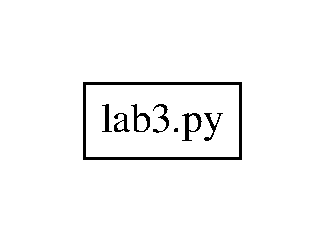
\includegraphics[width=0.5\textwidth]{figures/files}
%   \caption{\label{fig:files} Exercise files dependencies. In this lab, you
%   will be modifying \fileref{exercise3.py}, \fileref{ex3\_pendulum.py},
%   \fileref{exercise4.py} and \fileref{ex4\_hopf.py}.}
% \end{figure}

\section*{Coupled leaky integrator neurons}

\textit{The lab of today is based on a network of two coupled leaky-integrator
  neurons with self- connections as seen in the lecture, and as analyzed in the
  4 paper:
  \corr{\href{http://www.cs.uvm.edu/~jbongard/2014_CS206/Beer_CTRNNs.pdf}{Beer,
      R.D. (1995). On the dynamics of small continuous-time recurrent neural
      networks. Adaptive Behavior 3(4):469-509}}. By looking at the Figures
  4a-4d of that paper, you should be able to reproduce several interesting
  dynamical regimes and answer the questions below. See the file
  \fileref{lab3.py}}


\subsection*{5.a Set the parameters of the network such as to create a dynamical
  system with \textit{three} fixed points: two stable fixed points and one
  saddle node (check Beer 1995 for ideas and parameter values). Show figures
  that illustrate that behavior. Show or demonstrate the stability of the fixed
  points.}


\subsection*{5.b Set the parameters of the network such as to create a dynamical
  system with a limit cycle behavior and a single unstable fixed point. Show
  figures that illustrate that behavior. Look also at the behavior of the
  crossing of a Poincaré map (a line in this case). Discuss similarities and
  differences of this neural oscillator with the Hopf oscillator.}


\subsection*{5.c Set the parameters of the network such as to create a dynamical
  system with a limit cycle behavior and three fixed points: a single unstable
  fixed point, a single saddle node, and a single stable fixed point. Show
  figures that illustrate that behavior. Discuss similarities and differences
  with the Hopf oscillator. Discuss whether such a system could have interesting
  properties for motor control.}




\end{document}